\documentclass[12pt]{article}
\usepackage[utf8]{inputenc}
\usepackage{geometry}
\geometry{
 a4paper,
 total={170mm,257mm},
 left=20mm,
 top=25mm,
 }
\usepackage{layout}
\usepackage{amsmath, amssymb}
\usepackage{graphicx}
\usepackage{float}
\usepackage{pdfpages}
\usepackage[framed, numbered]{matlab-prettifier}

\setlength{\parskip}{1em}

\title{Checkpoint 2\\Telescopic Radio Antenna Design\\Design For Deflection Under Static Conditions\\Group 3}
\author{Shadan Amini\\Tate Halsey\\Serop Kelkelian\\Dominic Watson}
\date{\today}

\begin{document}
\pagenumbering{gobble}%
\maketitle
\newpage

\tableofcontents
\newpage

\section{Abstract}
\pagenumbering{arabic}
Our team has been tasked with designing a telescopic radio antenna to pick up (FM) signals for a portable radio. The goal of this report is to ensure that the material and geometry of the antenna is functional without fail, whilst satisfying the manufacturer’s design requirements. Approaching this specification with no restriction, the antenna is broken up into 6 segments. Upon full extension, the length of the antenna is 69.5 centimeters; fully retracted length measures out to approximately 11.5834 centimeters. Calculated tube wall thickness of the antenna is 0.0004167 centimeters, while the maximum diameter is 0.5 centimeter. In order to satisfy design requirements and functionality, the material chosen for this antenna was stainless steel 304. The density of the antenna comes out to 8000 $kg/m^3$ [2]. Calculating change in stress over change in strain, the elastic modulus of the antenna is 200 GPa [2]. The yield strength is 207 MPa [3]. Maximum normal stress for the antenna under a given loading is 167.815 MPa. The margin of security, or safety factor, for the antenna is 1.2335 (dimension-less). Maximum deflection was 0.06795 meters which occurred at the end of the antenna, at a length of 0.0695 meters. Total mass of the antenna comes out to 0.0182 kg. Total cost of raw materials needed to assemble the antenna was \$0.0042 USD.
\newpage

\section{Introduction}
We have been tasked to design a telescopic antenna that would serve as an (FM) signal receiver for portable radios. This task requires a specific design geometry must be chosen including number of sections, length, and thickness, that meet the given requirements and can successfully pick up FM radio signals. In [1], the frequency for (FM) radio signals ranges from 87 to 108 (MHz). To find the wavelength related to the frequency, the range of frequency was divided by the speed of light in a vacuum. The calculated wavelength for an (FM) radio signal ranges from 2.78 to 3.45 meters. Understanding that the design is a quarter-wave antenna and can only pick up one-quarter of the wavelength of the intended (FM) radio signal, the admissible length ($L$) for the antenna ranges from 0.695 to 0.8625 meters.
\newpage

\section{Design}

\begin{figure}[H]
\centering
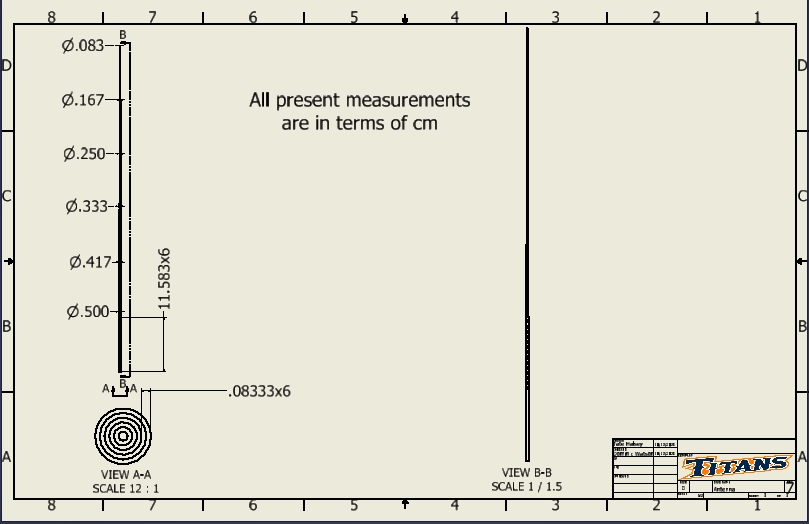
\includegraphics[height= 9.5cm, width= 14cm]{Antenna.png}
\end{figure}

The material chosen for this design is stainless steel 304. This material has a density of 8000 $kg/m^3$ [2], an elastic modulus of 200 GPa [2], and a yield strength of 207 MPa [3]. The antenna design has 6 segments that are all 11.583 centimeters in length, for a total length of 69.5 centimeters. The segments decrease in radius moving upwards by a factor of 0.04167. The diameter of the largest segment is $0.5$ centimeter.
\newpage

\section{Static Stress Analysis}
In the process of deriving our static stress analysis, there were a plethora of problems to be solved leading to our result. The given free-body diagram, \Cref{Figure 1} helped create a shear-force and bending-moment diagram, \Cref{Figure 2} and \Cref{Figure 3}, respectively.

\begin{figure}[H]
\centering
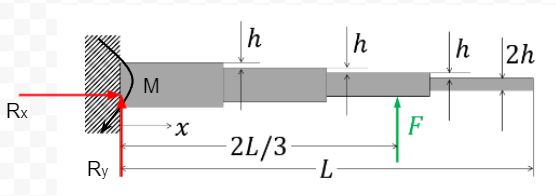
\includegraphics[height= 4cm, width= 10.5cm]{freebody.png}
\caption{Free Body Diagram}
\label{Figure 1}
\end{figure}

\begin{figure}[H]
\centering
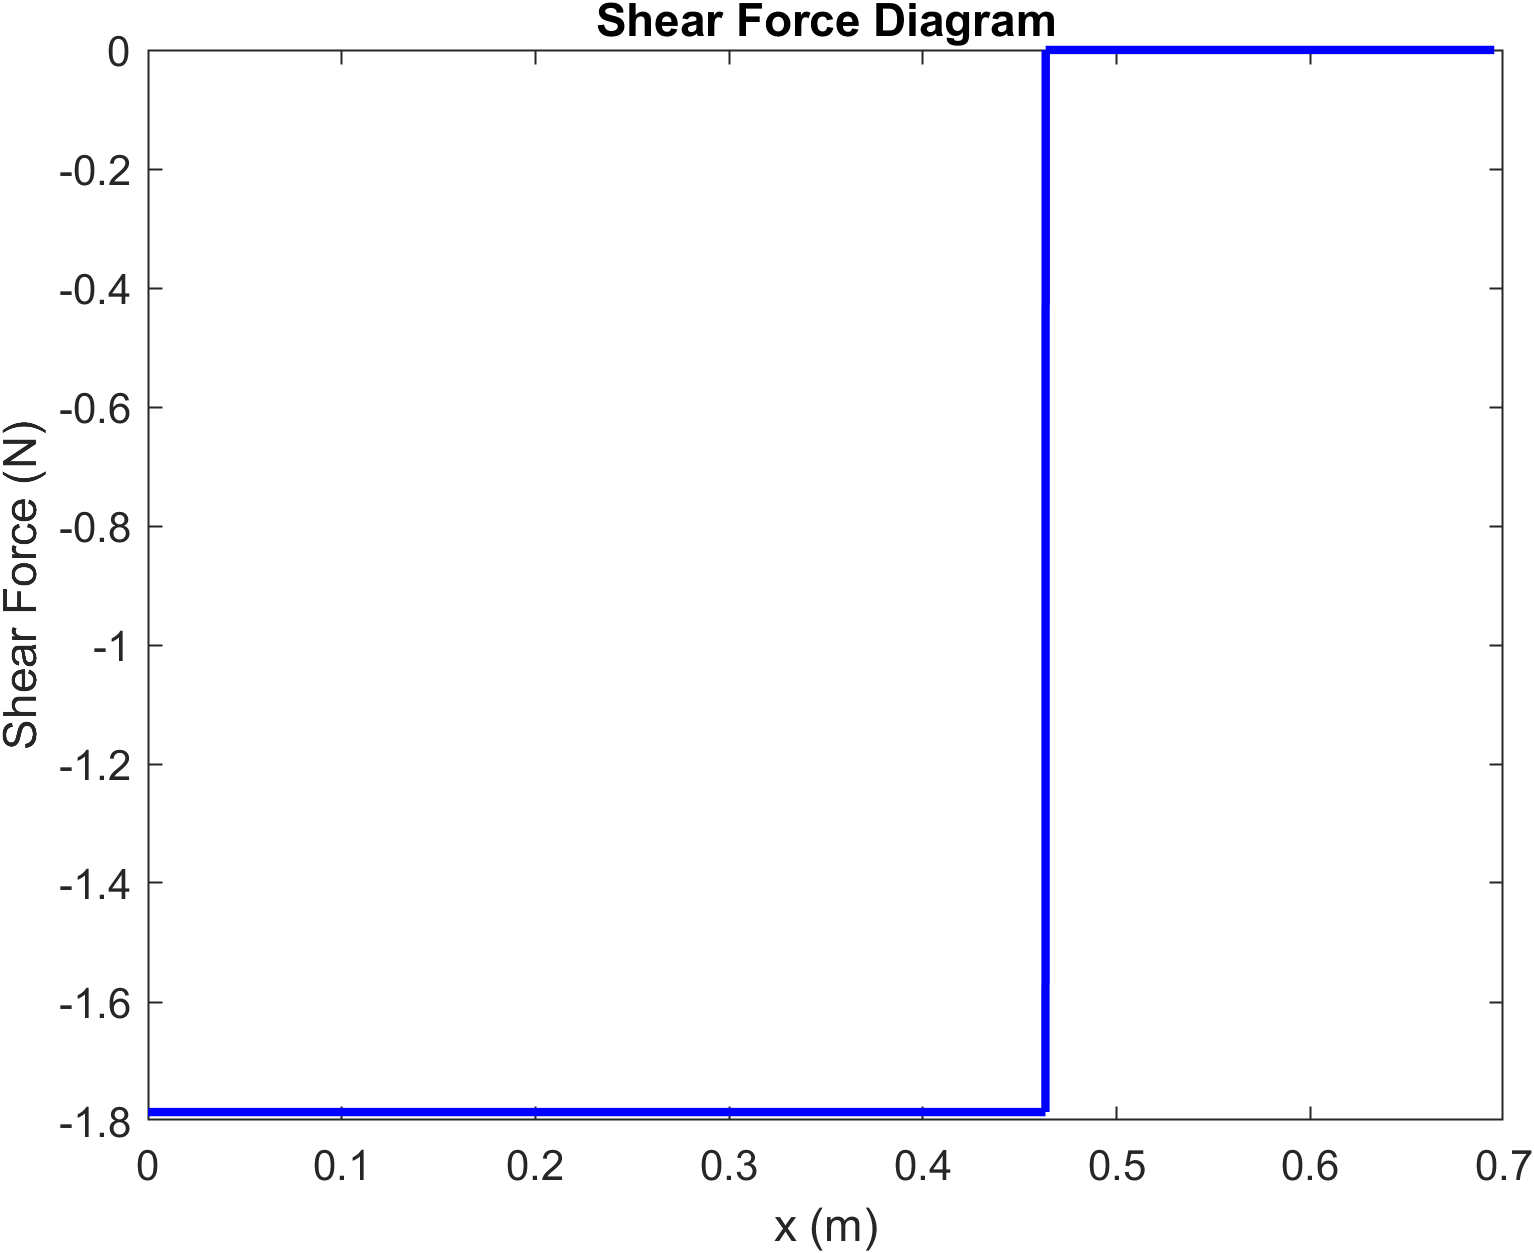
\includegraphics[height= 9.5cm, width= 12.5cm]{curve_Shear_Force.png}
\caption{Shear Force Diagram}
\label{Figure 2}
\end{figure}

\begin{figure}[H]
\centering
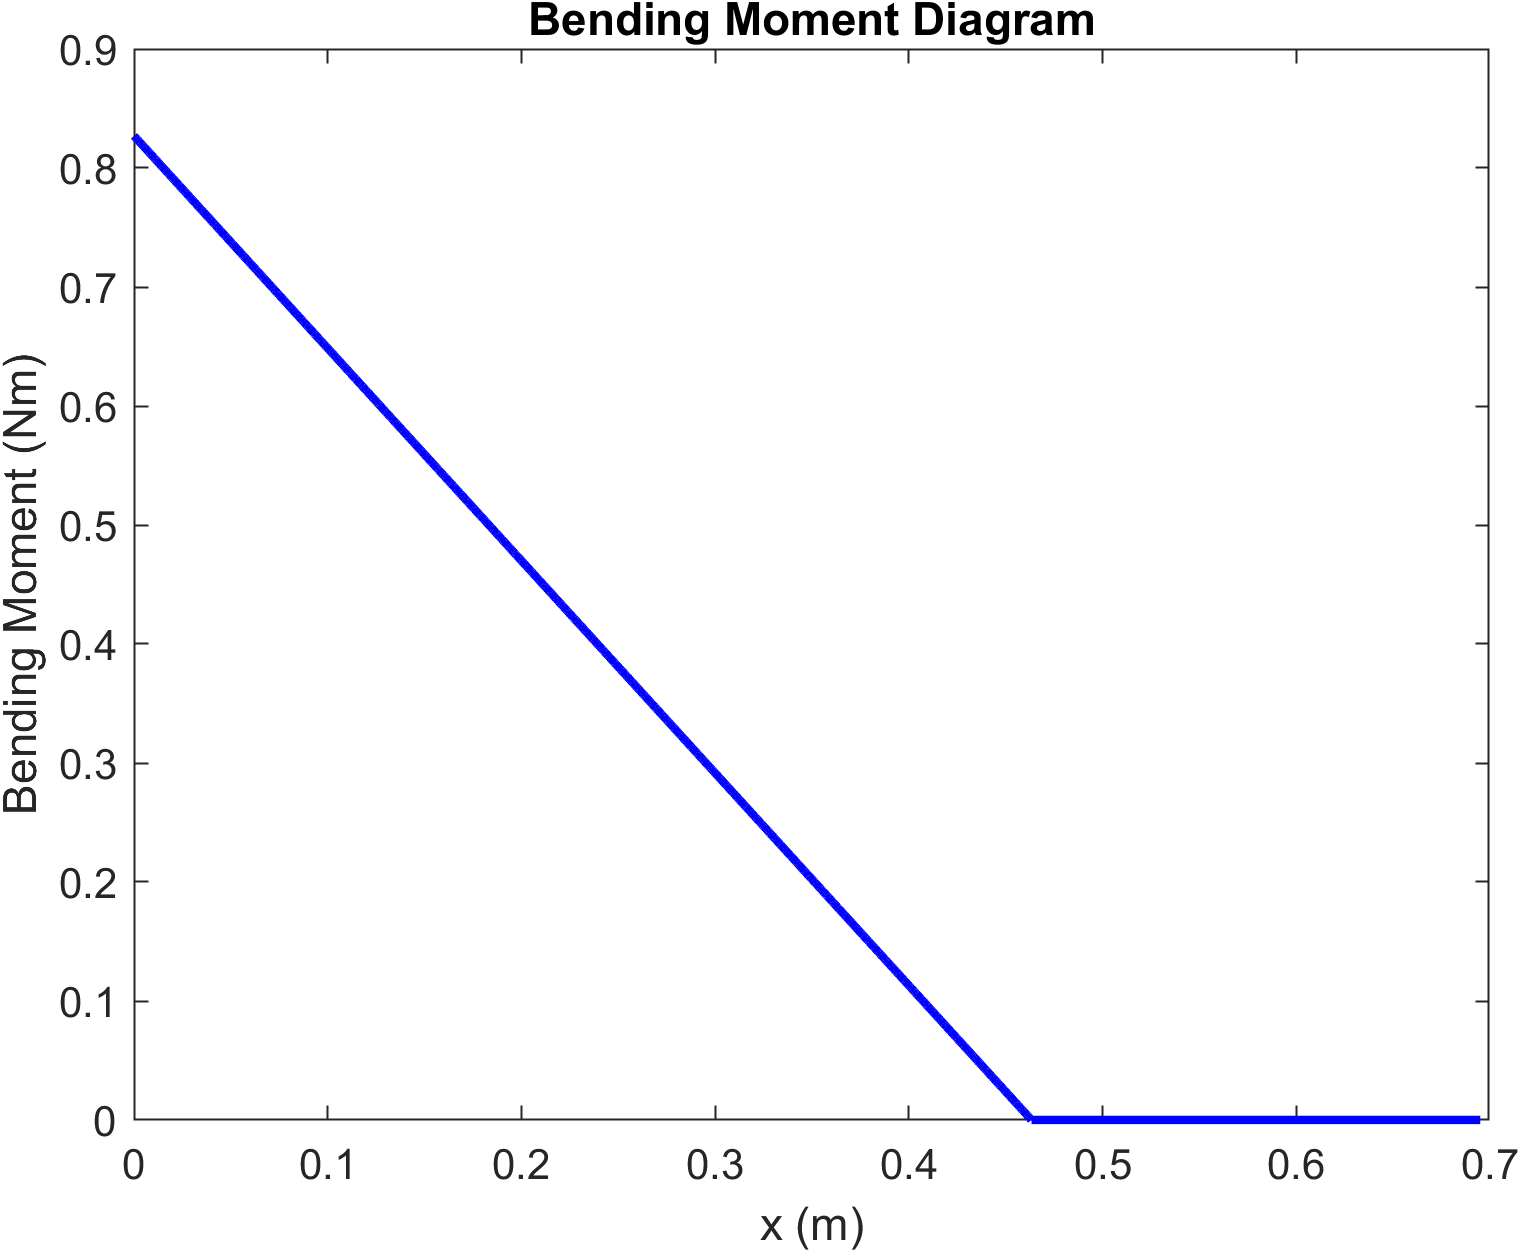
\includegraphics[height= 9.5cm, width= 12.5cm]{curve_Bending_Moment.png}
\caption{Bending Moment Diagram}
\label{Figure 3}
\end{figure}

\setlength{\parindent}{0cm}
This stage was simply recognizing that the arbitrary concentrated force $F$ was the single external force acting on the beam, so the only internal reaction force $R_y$ must be equal in magnitude but opposite in direction as to maintain static equilibrium. This concept stayed relevant in the bending moment diagram as well for the only moment was caused by the single concentrated force F at a distance $2L/3$, where $L$ is the full length of the antenna and is equal to 0.695 meters, therefore there must be a moment at the support equal in magnitude but opposite in direction to maintain static equilibrium. Now with this first step out of the way, the next step was to derive a symbolic equation for $M(x)$ using the Laplace transform technique. 

Originally, we were given the equation
\begin{equation}
    \centering
    \ M''(x) = w(x),
\end{equation}
where $M''(x)$ is the second derivative of the bending moment with respect to x and $w(x)$ is the transverse force per unit length applied to the antenna as a function of x.

After deciding on a form for $w(x)$  to take, our work arrived us to
\begin{equation}
    \centering
    \ w(x) = F\delta(x - \frac{2L}{3}).
\end{equation}
We then took the Laplace transformation of both sides, resulting in
\begin{equation}
    \centering
    \ s^2 \mathcal{L}[M(x)] - sM(0) - M'(0) = \mathcal{L}[w(x)].
\end{equation}
After inputting values gained from the bending moment graph, move appropriate values to the right side of the equation and arrive at the equation
\begin{equation}
    \centering
    \ s^2 \mathcal{L}[M(x)] = F\mathcal{L}[\delta(x - \frac{2L}{3})] + \frac{2FL}{3}{s} - F.
\end{equation}
At this point we are left with solving for the Laplace of the $w(x)$  function
\begin{equation}
    \centering
    \   s^2 \mathcal{L}[M(x)]=Fe^{-\frac{2L}{3}} + \frac{2FL}{3}{s} - F.
\end{equation}
Then divide both sides by $s^2$,
\begin{equation}
  \centering
  \mathcal{L}[M(x)] = \frac{Fe^{-2L/3 \cdot{s}}}{s^2} + \frac{2FL}{3} \cdot \frac{1}{s} - F \cdot \frac{1}{s^2}
  \end{equation}
 and take the inverse Laplace of both sides,
 \begin{equation}
  \centering
   M(x) = {F\mathcal{L}}^{-1}(\frac{e^{-2L/3 \cdot{S}}}{s^2}) + \frac{2FL}{3} \cdot \mathcal{L}^{-1}(\frac{1}{s})- F\mathcal{L}^{-1} (\frac{1}{s^2}).
  \end{equation}
 Finally, solve for the bending moment equation $M(x)$,
  \begin{equation}
  \centering
   M(x) = -Fx + \frac{2FL}{3} + F(x - \frac{2L}{3}) \cdot H(x - \frac{2L}{3}),
  \end{equation}
  where $F$ is the concentrated force, $L$ is the length of the antenna, and $H(\;)$ is the Heaviside function.
  
Once the derivation was complete, it was onto plotting the relevant equations for the maximum normal stress. The maximum vertical distance from the neutral surface within the cross-section, $C(x)$ is found in \Cref{Figure 4} and given by the equation,
\begin{equation}
  \centering
   C(x) = Nh-h \cdot{H(x - \frac{n \cdot{L}}{N}}),
  \end{equation}
where $N$ is the number of segments present on the antenna, $h$ is the thickness of each antenna piece, and $n$ is an arbitrary variable used for the iterable.

Next is $I(x)$, seen in figure 5, which is the second moment of area of the cross-section and given by the equation:
\begin{equation}
  \centering
   I(x) = I - \frac{\pi}{4}h^4((N - n + 1)^4 - 2(N - n)^4 +(N - n - 1)^4)H(x - \frac{n\cdot{L}}{N}).
  \end{equation}
 Finally, the normal stress $σ(x)$ shown in \Cref{Figure 6}, is given by the equation,
 \begin{equation}
  \centering
   \sigma(x) =  \frac{|M(x)|C(x)}{I(x)}.
  \end{equation}
  With both these graphs available for inspection and their necessary code refined, important pieces of data can be found. One of interests is the location of the maximum normal stress, which occurred at the length 0.3475 meters, therefore the exact numerical value for normal stress is given by the equation,
  \begin{equation}
  \centering
   \sigma(x) = \frac{|-Fx + \frac{2FL}{3} + F(x - \frac{2L}{3})H(x - \frac{2L}{3})|Nh - h \cdot H(x -\frac{n \cdot{L}}{N})}{I - \frac{\pi}{4}h^4((N - n + 1)^4 - 2(N - n)^4 +(N - n - 1)^4)H(x - \frac{n\cdot{L}}{N})},
  \end{equation}
  when x is equal to 0.3475 meters. Then once inputted with appropriate constants, it resolves into approximately 1.6781\cdot$10^{8}$ Pa. With this approximate value our safety factor is found to be 1.2335 (dimension-less).

\begin{figure}[H]
\centering
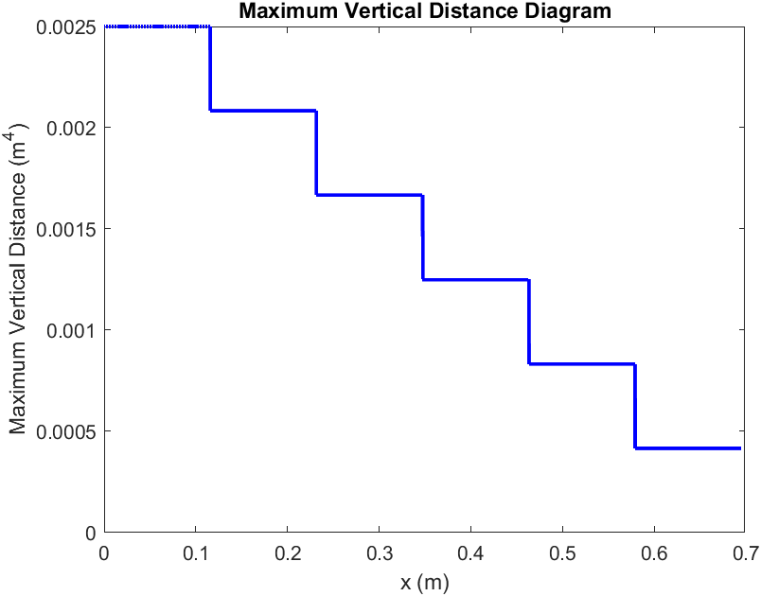
\includegraphics[height= 9.5cm, width= 12.5cm]{Max_Vertical_Distance.png}
\caption{Maximum Vertical Distance}
\label{Figure 4}
\end{figure}

\begin{figure}[H]
\centering
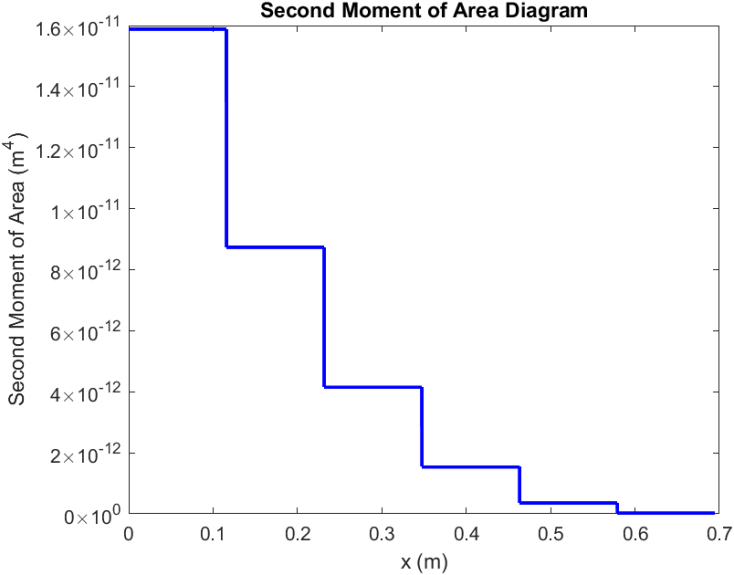
\includegraphics[height= 9.5cm, width= 12.5cm]{Second_Moment_of_Area.png}
\caption{Second Moment Area}
\label{Figure 5}
\end{figure}

\begin{figure}[H]
\centering
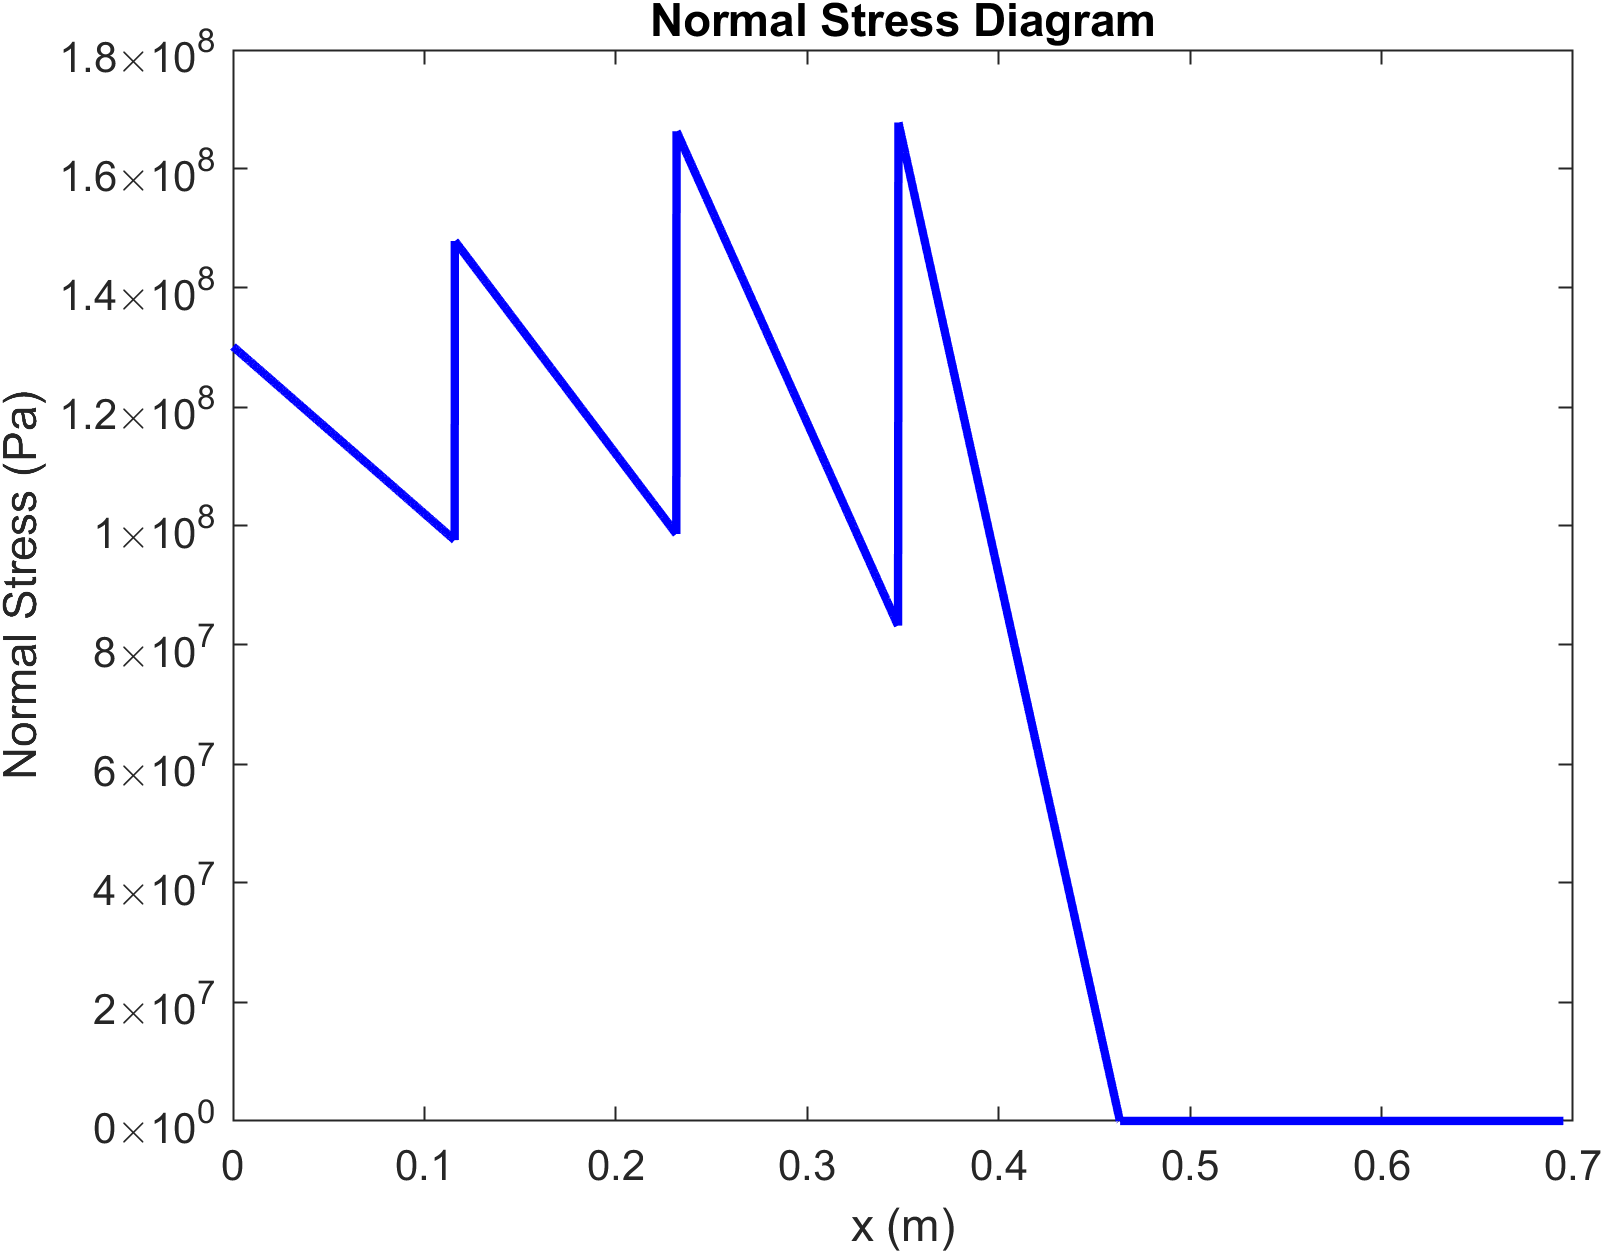
\includegraphics[height= 9.5cm, width= 12.5cm]{curve_Normal_Stress.png}
\caption{Maximum Normal Stress}
\label{Figure 6}
\end{figure}
\newpage

\section{Static Deflection Analysis}
While analyzing deflection under static conditions, we solved for the deflection curve using the Euler-Bernoulli beam equation. In order for the deflection curve to be the solution to the Euler-Bernoulli beam equation, the assumptions of Euler-Bernoulli beam theory must be met. First, the cross-sections must remain planar and normal to the longitudinal axis before and after deformation. Because it does not deform permanently, the cross-section is considered a rigid surface which means it can only rotate. The second assumption is that the beam is homogeneous and has a longitudinal plane of symmetry. Lastly, even though the beam has a slight curve after deformation, deflections are considered to be small and shear deformations are to be neglected.
\setlength{\parindent}{0cm}

Because these assumptions are met, we could use
\begin{equation}
    \centering
    \ EI(x)u''(x) = M(x),
\end{equation}
the Euler-Bernoulli beam equation to solve for the deflection curve. Here $E$ is the modulus of elasticity, $I(x)$ is the second moment of area, and $M(x)$ is the bending moment.

Isolating $u’’(x)$, we obtain 
\begin{equation}\label{eq:Deflection}
    \centering
    \ u''(x) = \frac{M(x)}{EI(x)}.
\end{equation}
The antenna is being modeled as a cantilevered beam as the antenna is fixed on the supported end. The boundary conditions at $x = 0$ are given below:
\begin{equation}
    \centering
    u(0) = 0,\; \;u'(0) = 0.
\end{equation}
Solving for this problem analytically is much more difficult than solving numerically because $I(x)$ and $M(x)$ are both piecewise functions and as $N$, the number of segments grows increasingly large.

The procedure for Euler’s method goes as follows. First, one must identify the dependent and independent variables. We are using Euler’s method to solve for the vertical deflection as a function of $x$, distance along the length of the beam. Thus, the independent variable is $x$ and the dependent variable is the vertical deflection. Next, we must discretize the independent variable. In this case, we will discretize $x$ into constant increments of $x$. After discretizing the independent variable, approximate all derivatives with finite difference quotients. We are solving for vertical deflection with respect to $x$. As the constant increments of $x$ get smaller, the approximation becomes more accurate because the numerical solution will get closer and closer to the analytical solution. Using a sufficiently small increment $\Delta{x}$, we could successfully model the behaviour of $u(x)$ everywhere. After modeling the behaviour of $u(x)$, use this equation 
\begin{equation}\label{eq:Eulersmethodu}
    \centering
    u_{n+1} = {u_n}\;+u_n'\; \Delta{x}
\end{equation}
to solve for quantities at $(n+1)^{th}$ time step in terms of quantities at the $n^{th}$ time step. In Equation~\eqref{eq:Eulersmethodu}, $u_{n+1}$ is the quantity at the subsequent time step, $u_n$ is the quantity at the previous time step, $u_n'$ is the derivative of the quantity at the previous time step and $\Delta{x}$ is the length increment. Taking the derivative of both sides of the equation gives us
\begin{equation}
    \centering
    u_{n+1}' = u_n'\;+u_n''\; \Delta{x}
\end{equation}
which we use in the for loop to calculate the deflection curve. Because this equation is used in the for loop, it will be iterated over from 0 to the length of the antenna incrementing by $\Delta{x}$. This makes it very time-efficient to solve this problem numerically using MATLAB. After constructing a numerical solution, we will run a convergence study to ensure that our numerical solution converges to the analytical solution. We will decrease $\Delta{x}$ by orders of magnitude until the numerical solution stops changing to the desired accuracy.

Once the derivation was complete, we modified the MATLAB script to include the deflection curve. The deflection curve was created to identify the single greatest deflection $|u|_{max}$ along the entire length of the antenna, and the point at which that deflection occurs. 

Using an exact increment, 
\begin{equation}
    \centering
    \Delta{x} = 0.0001;
\end{equation}
we obtained a deflection curve shown in \Cref{Figure 7}. According to \Cref{Figure 7}, the greatest deflection was 0.067095 meters which occurred at a length of 0.695 meters. This is equal to the maximum value specified for the length of the antenna in the design requirements.

\begin{figure}[H]
\centering
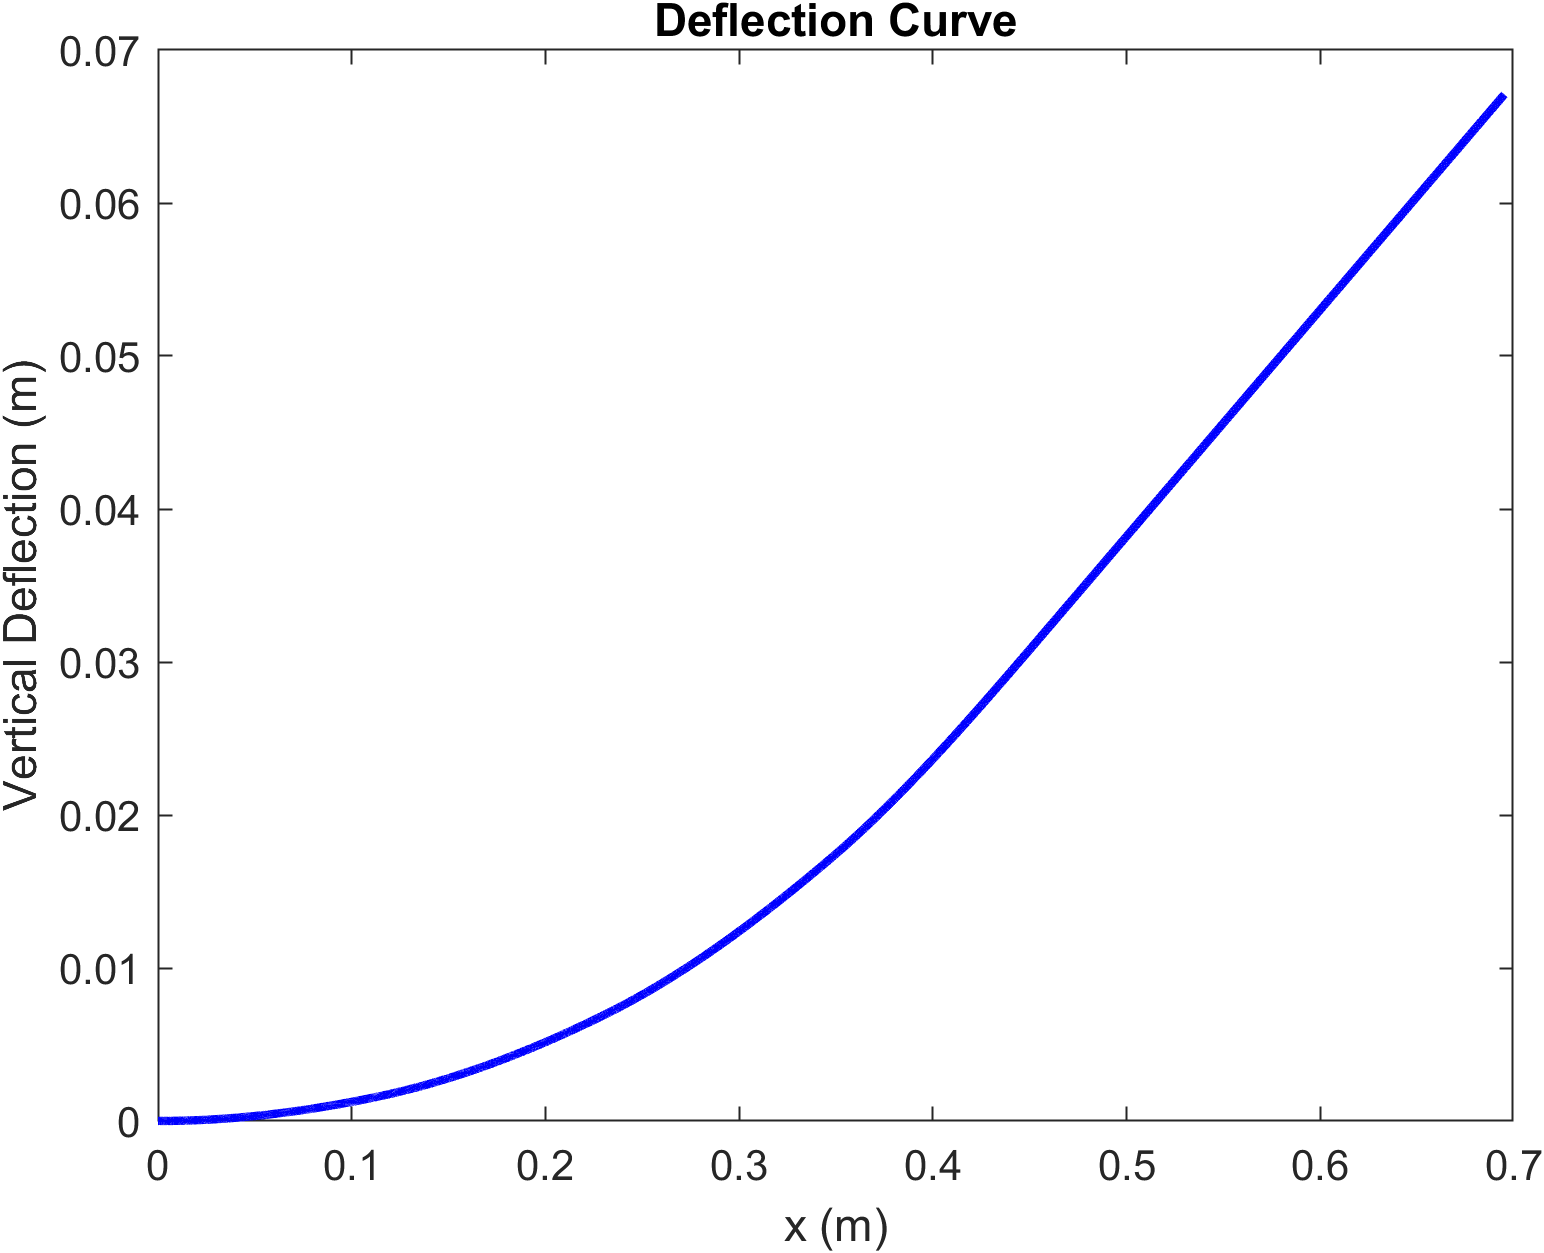
\includegraphics[height= 9.5cm, width= 12.5cm]{curve_Deflection_Curve.png}
\caption{Deflection Curve}
\label{Figure 7}
\end{figure}
\newpage

\section{Cost}
The total mass of the antenna is 0.0182 kilograms. This was calculated by multiplying the density times the volume. The cost of stainless steel is approximately \$0.23 per kilogram [4]. The cost of the stainless steel for the antenna design is \$0.0042.
\newpage

\section{Conclusion}
For the antenna design the material that was used is stainless steel 304. Stainless steel 304 has a density of 8000 $kg/m^3$ [2], an elastic modulus of 200 GPa [2] and a yield strength of 207 MPa [3]. Geometrically, this design has 6 segments. When fully extended the length of the antenna is 69.5 centimeters and when fully retracted the length is 11.583 centimeters. The tube wall thickness is $4.1667 \cdot{10^{-2}}$ centimeters, and the maximum diameter is 0.5 centimeters. The cost of the raw material is \$0.0042 with the mass of our antenna being 0.0182 kilograms. The maximum normal stress under given loading is 167.815 MPa. The maximum deflection under given loading is 0.06795 meters. With a concentrated force of 1.7849 Newtons acting at 46.333 centimeters from the fixed end of the antenna, the factor of safety is 1.2335 (dimension-less). While choosing the design, we wanted to minimize cost while maintaining a design that had a factor of safety of at least 1.2. When finding the geometry, the length was decreased to the lowest length that can still permit an FM radio signal and determined $h$ by dividing the radius by the number of segments. By inputting different numbers of segments, we were able to monitor the change in the factor of safety and come to a lower value that still meets design parameters. Problems that were encountered while working on the project were mostly mathematical, as well as issues incorporating that math into working code on MATLAB. Possible improvements include looking at a larger sample of materials and finding a cheaper cost that still satisfies design requirements and the requirements for an FM radio signal.$
\newpage

\section{References}
[1] Y. Zhang, Z. Yang, L. Deng and S. Li, “Research on Wireless Positioning Technology Based on Digital FM Broadcasting”, International Journal of Digital
Multimedia Broadcasting, vol. 2019, Article ID 1051386, 10 pages, 2019.v

[2] H. M. Cobb, “History of Stainless Steel: Two New Classes
of Stainless Steel.” 1st ed. Ohio: A S M International, 2010.

[3] Thyssenkrupp Materials LTD, C. Lane, C. Heath, West    Midlands, “Stainless Steel 304 1.4301,” Jan. 2018. Accesses on: Oct. 11, 2021. [Online]. Available:          https://www.thyssenkrupp-materials.co.uk/stainless-steel-304-14301.html

[4] “Stainless Steel: 304 SS,” [Online]. Available: https://www.scrapmonster.com/scrap/304-ss/48
\newpage

\section{Appendix A: Design Specification Form}
\begin{figure}[H] 
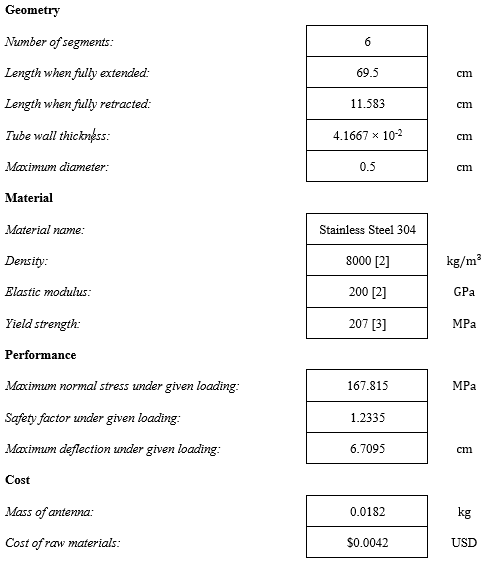
\includegraphics[height= 21.5cm, width= 17.5cm]{Appendix_A.png}
\end{figure}
\newpage

\section{Appendix B: Authorship Declaration Form} 
\begin{figure}[H]
\centering
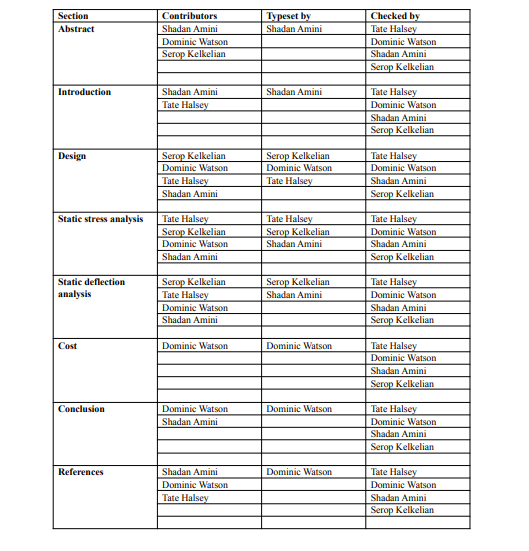
\includegraphics[height= 20.5cm, width= 18.5cm]{AuthorDec.png}
\end{figure}
\newpage

\section{Appendix C: MATLAB Script}
\lstinputlisting[style = Matlab-editor]{projectScripts.m}
\newpage

\end{document}